\providecommand{\heading}[1]{\section{#1}}
\providecommand{\subheading}[1]{\subsection{#1}}

\heading{Participants}
    All participants in this experiment were students taking CS 561 System Defense and Test.

    \subheading{Course Information}
        The course CS 561 is a cybersecurity course offered to both undergraduate and graduate students through the University of Massachusetts Amherst. %%
The course specifically focuses on offensive security and penetration testing. %%
Much of the course work revolves around highly prescriptive hands-on activities described in the book \textit{Penetration Testing: A Hands-On Introduction to Hacking} by Georgia Weidman. %%
The course description for CS 561 states:

        \begin{quote}
            This class trains students to detect and analyze weaknesses and vulnerabilities in target systems as a method of assessing the security of a system. %%
We focus on tools and techniques that an attacker would employ but from the perspective of an ethical system administrator. %%
Topics include tools and techniques for penetration testing and attacks, information gathering, social engineering, and defenses. %%
Specific topics include malware, denial of service attacks, SQL injection, buffer overflow, session hijacking, and system hacking, network sniffing and scans, wireless encryption weaknesses and other WiFi issues, IDS/firewall evasion, metasploit tools, physical security, and setting up honeypots. %%
Was INFOSEC 690S. This course counts as an Elective toward the CS Major.

            Undergraduate Prerequisites: COMPSCI 460 (or COMPSCI 597N or COMPSCI 660) and COMPSCI 453. %%
3 credits.
        \end{quote}
        \noindent
        To enroll in the class, students are required to have knowledge of computer networks, and network security. %%
Undergraduates must have taken courses in this area ---%%
 CS 453 teaches computer networks; %%
CS 460, 597N and CS 660 all teach network security. %%
Graduate students are expected to have prior knowledge in these areas. 

\heading{Student Surveys}\label{sec:blank-surveys}
\subheading{Survey 1: Crypto Cracking}\label{subsec:blank-surveys-cc}
\noindent
    The following survey was given to students to fill out after completing the \say{Crypto Cracking} activity.
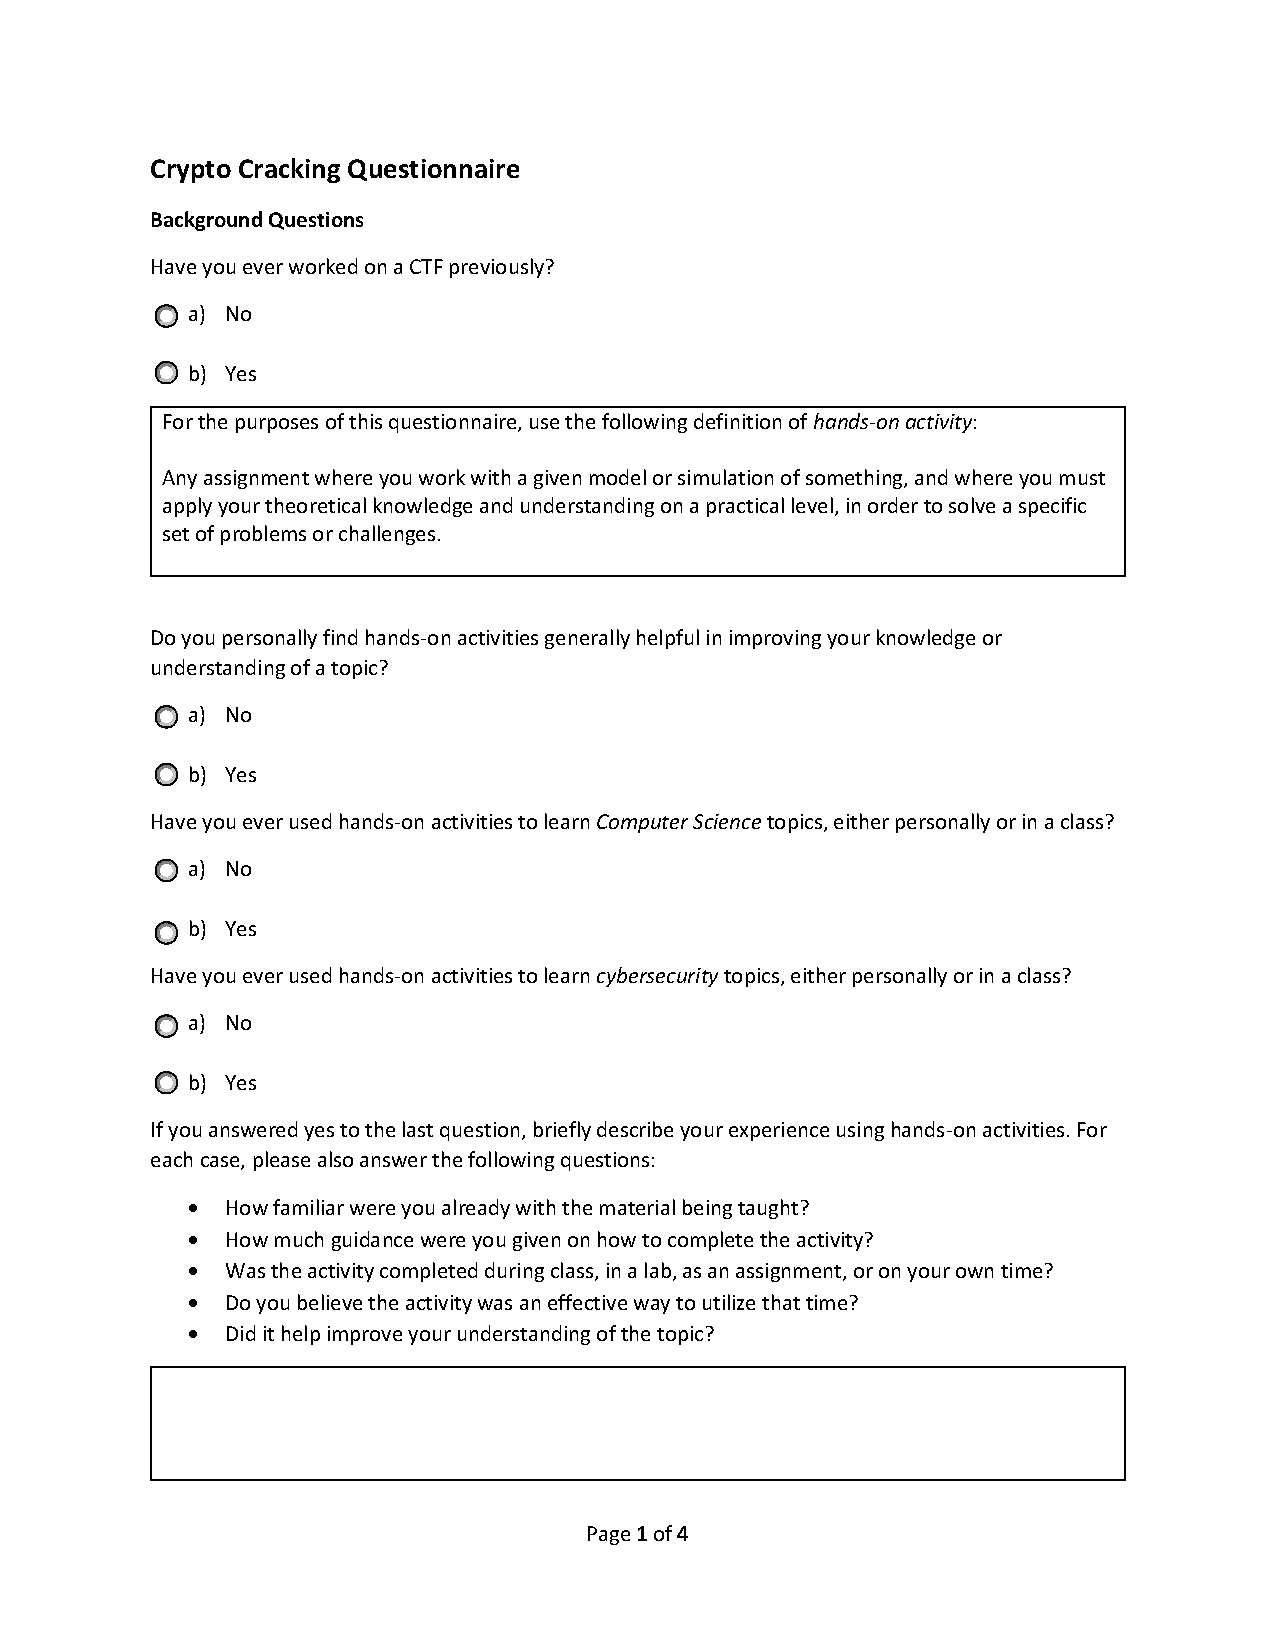
\includepdf[pages=-]{../CTF-Surveys/survey1-cc.pdf}

\subheading{{Survey 2: Going Backwards}}\label{subsec:blank-surveys-gb}
\noindent
    The following survey was given to students to fill out after completing the \say{Going Backwards} activity.

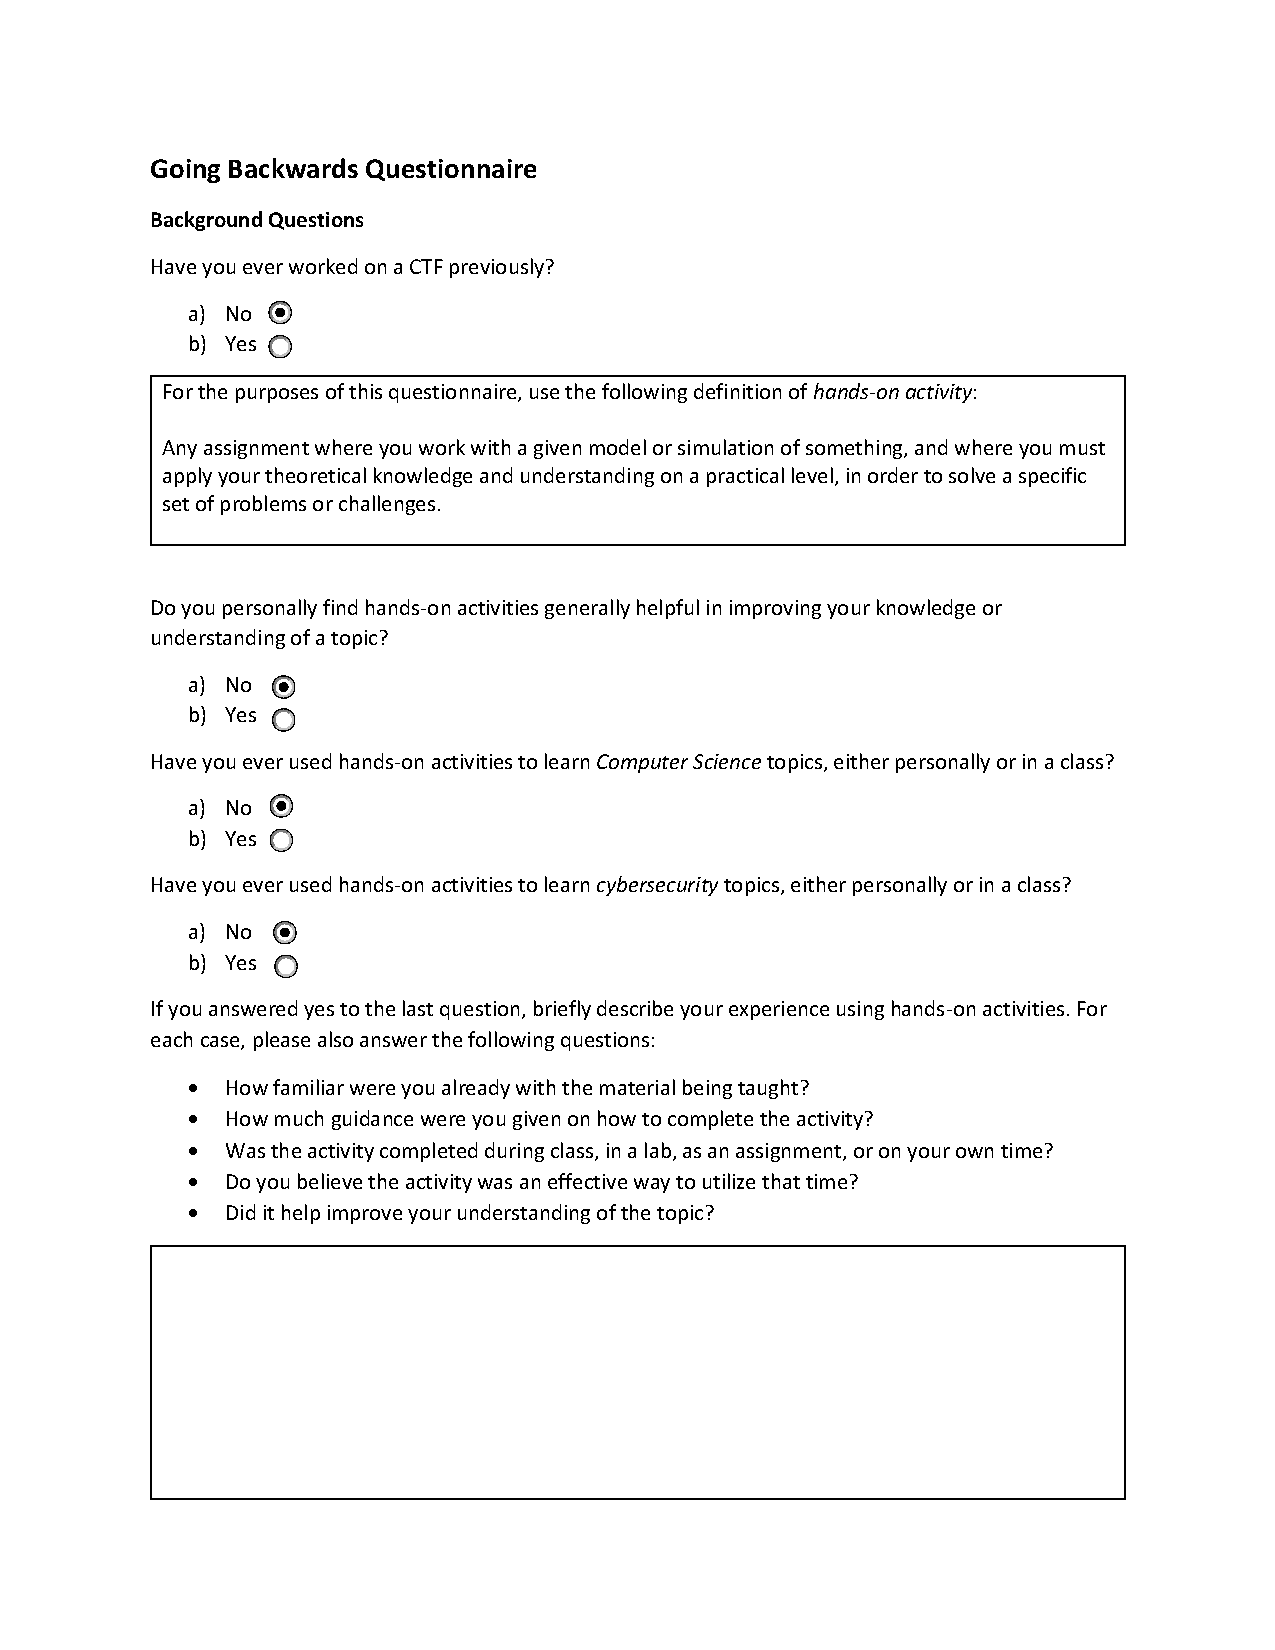
\includepdf[pages=-]{../CTF-Surveys/survey2-gb.pdf}

\heading{Student Responses}
